\appendix
\chapter{Sustainability and costs}

This project was carried out by a single student, which means the cost of it was very low. However, a project that depends on students is not a sustainable one since students are highly underpaid. For that reason I would like to provide a quantitative analysis on the real costs of carrying out this work. 

Let's start counting the hours of work required to just build the dataset. Even after using a semi-automatic procedure to label the data, many hours were needed to end up with 85 labelled images. Roughly 100 hours of human labour and 20 hours of compute power were employed to create segmentations. Another 15 hours of expert human labour were required to review the class annotations by the physician. Now, let's translate that into money. The first 100 hours required very low training, just the ability to paint circles. A fair salary for that can be 10€/h (if outsourced it could be less than 2€/h). That translates into a cost of 1000€. The compute power requires GPUs that consume at most 350W. Let's estimate the CPU, memory and GPU consumption by 300W on average, which means $4.5$kWh were consumed. That means $0.93$€ if the price of electricity is $0.15$€/kWh. And the expert work is typically paid more, let's estimate 20€/h which means 300€ in total. The total cost of creating the database would be $1300.93$€. If we divide by the number of images we have a total of $15.30$€ per image. 

Second, the salary of the technical workers. A project like this normally requires a software developer, a data engineer and a project manager. Depending on the experience the salaries may range. For simplicity, let's consider the software developer is junior (30K/year), the data engineer is senior (50K/year) and the project manager has nearly five years of experience (80K/year). Assuming the project is carried out in just one year, and taking into account the extra 30\% that needs to be payed to the social security, the total cost in salaries would be $208000$€.

Third, putting a machine learning model in production is more than just creating it. It needs to be maintained, and someone has to care about the drift. Models performs worse when time passes because the data distribution is not fixed. New patients means new training is needed. Hospitals would need to train their technicians to perform retrainings and physicians to relabel. The cost of relabelling is already estimated: $15.30$€ per image. Remains to estimate the cost of training technicians. 385\$ or 350€ per person is what a course on machine learning would cost\footnote{\url{https://www.ml.school/c/start-here} Accessed 8th April 2023}.

Finally, to show that the project is sustainable, it has to generate some value. I believe in open science and medicine. Putting a price in other people's lives is not ethical, so privatising this project is not an option. But someone has to pay the cost, in this case, the government. A project like this is only sustainable if public opinion is in favour of it. More data is needed to exactly estimate the social value this will bring. In my opinion, this product will reduce physician workloads, which is beneficial. By reducing the workload, the diagnostic process can be accelerated, and receiving faster diagnostics is something the public opinion will definitely be interested about.

\chapter{The problem of merging cells}\label{sec:merge_cells}

One of the problems that appeared when using Hovernet was broken cells. In many cases, big cells were predicted as various small cells. It is visually appalling and that is why we designed an algorithm to merge broken cells. The result is on \autoref{fig:morph_}.

\begin{figure}[ht]
\begin{subfigure}[b]{1\textwidth}
    \centering
    
\includegraphics[width=\textwidth]{imgs/morph1.png}
    \caption{Before}
    \label{fig:morph1}
\end{subfigure}
\begin{subfigure}[b]{1\textwidth}
    \centering
    
\includegraphics[width=\textwidth]{imgs/morph2.png}
    \caption{After}
    \label{fig:morph2}
\end{subfigure}
\caption{Example of cells that were not fully detected by Hovernet. After applying our algorithm all the smaller cells were merged into one.}
\label{fig:morph_}
\end{figure}

The algorithm leverages techniques of mathematical morphology. If we call $X_1$ the image predicted and $X_2$ the image that identifies the background with the value zero and the rest with one, then, the image $(\delta (X_1) - X_1)  \cdot X_2$ contains the frontiers of the cells, being $\delta$ a dilation. An illustration of the process is on \autoref{fig:morph}.

\begin{figure}[ht]
    \centering
    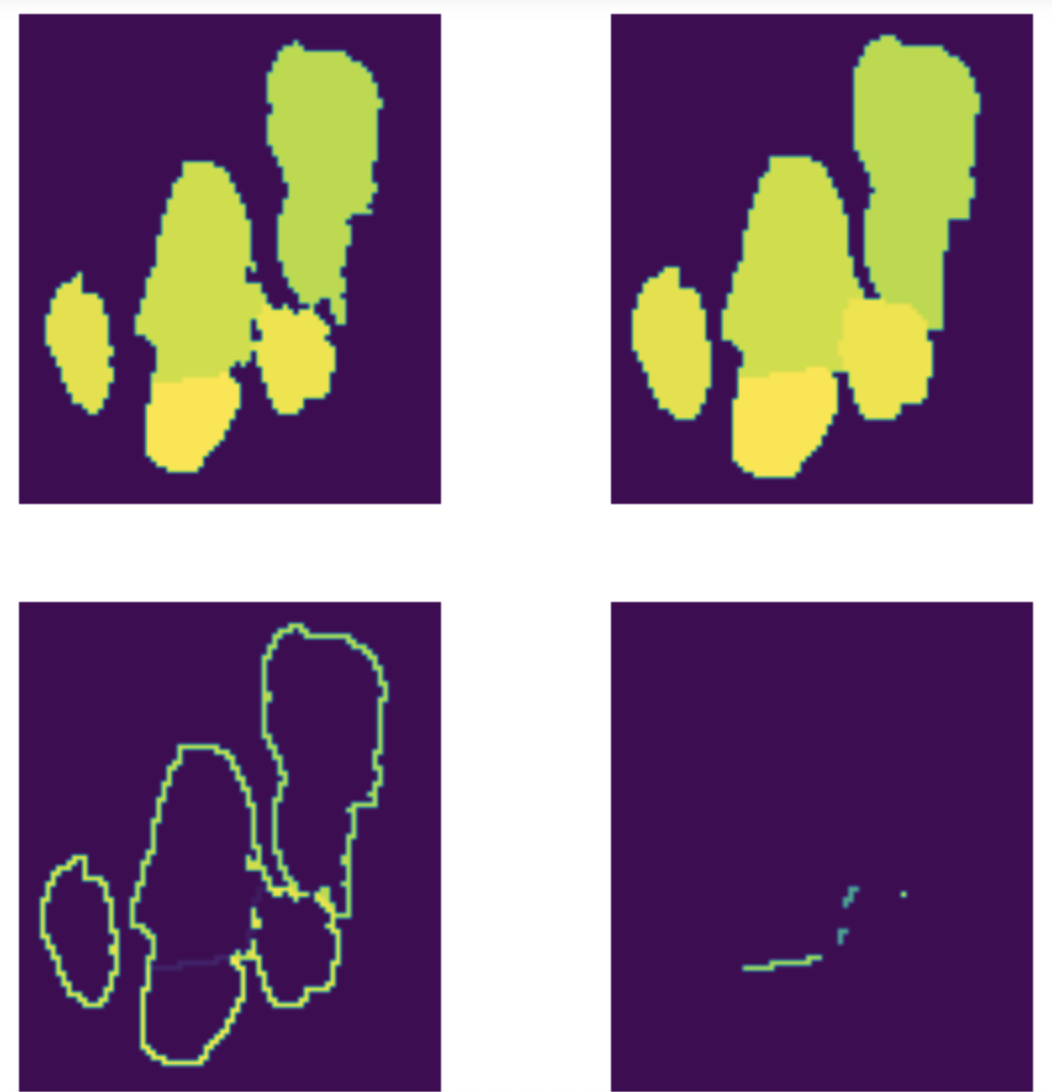
\includegraphics[width=0.5\textwidth]{imgs/morphInflam.png}
    \caption{Top-left is the original image, top-right is the dilation, bottom-left the gradient and bottom-right the masking which is the final result.}
    \label{fig:morph}
\end{figure}

The problem here is that different frontiers may end up with the same identifier. $X_1$ contains the identifier of each cell in every pixel of such cell. But, $(\delta (X_1) - X_1)  \cdot X_2$ contains the differences of identifiers in the position of the frontier. Differences of different pairs may end up with the same value. E.g.: $4-3 = 2-1$. To solve that, it is needed to properly set the identifiers so that each pair can be uniquely identified by the difference between the maximum and the minimum. One simple solution to that is to use powers of two. More concretely, applying the function $n \mapsto 2^n$ to the identifiers. This way $2^n-2^m$ is a function that can be inverted back to the pair $(n,m)$ where $n>m$. However, we can have up to 1500 cells, requiring identifiers up to $2^{1500}$ is clearly unfeasible and is not compute optimal since to identify pairs we only need $1500 \choose 2$ $=1.124.250$ identifiers. The best function I have found so far is $n \mapsto n^5$, using other simple lower degree polynomials doesn't uniquely identify the difference for values up to 1500 \cite{4567383}.

\chapter{TumourKit}

The whole thesis dealt with the theory and the results of the experiments. Behind all that there was a lot of software needed to make it all work. I decided to build a python library that other people could use to replicate my experiments and design new ones. The library is called TumourKit. The code is available on GitHub\footnote{\url{https://github.com/Jerry-Master/lung-tumour-study}} under the Affero GPLv3 license. It is tested on Ubuntu and Windows for python versions 3.8, 3.9 and 3.10. It has more than ten thousands lines of code, counting comments. For a more detailed explanation on how to use it and what is offered, please, read the docs\footnote{\url{https://lung-tumour-study.readthedocs.io/en/latest/}}.

\chapter{Soft Labels}

One of the problems we encountered when reviewing the lung dataset was that the expert was not sure which label to give to some cells. It was solved by simply ignoring those cells since in practice it didn't really matter because we are interested in percentages and a cell with no label can be removed from the numerator and denominator. However, we do preserve that information in the dataset because it could be used to train the models with soft labels. Even though we didn't try it, we expect it could help further calibrate the resulting probabilities. For that reason, in this appendix I will be explaining how to adapt all the methods presented in the thesis to soft labels. 

The easiest ones to adapt are the graph neural networks. They are trained using the softmax, so they are already compatible with soft labels. It is only needed to substitute the one hot encoded vector of labels to a vector of probabilities and everything works exactly the same.

The XGBoost method requires a little trick. Although XGBoost also uses softmax for training, current implementations threshold the label so providing probabilities is of no use since the soft labels will be made into hard labels. Nonetheless, XGBoost supports a weight for each row in the dataset. This makes it possible to use the probabilities as weights. The trick consists of repeating rows one time for each class and assign that class probability to that repeated row weight. The idea was taken for an online forum\footnote{\url{https://stackoverflow.com/a/66481600}} and the explanation behind how this works is that XGBoost multiplies the gradient and hessian by the weight and not by the label, as explained in another online forum\footnote{\url{https://stats.stackexchange.com/a/365555/378093}}. 

The trickiest method to adapt is HoVerNet. Having soft labels does not affect neither the HV branch nor the NP branch but it does affect the NC branch. That branch is trained using the softmax and the dice loss. The first one is quite easy to adapt as described for the graph neural networks. However, the dice loss requires more thinking. In Zifu Wang et al. \cite{wang2023dice} they propose a way of extending the dice loss for soft labels with promising results. On a more technical and practical level, modifying the codebase to support this metric is too much of a hurdle given the expected benefits. But it is interesting on a theoretical perspective to know of the existence of such possibility. In the future, when it becomes a more refined technique with wider support on the main libraries, it may be a good way of training better models.